% Arquivo LaTeX de modelo de dissertação/tese a ser apresentados à CPG do Museu de Zoologia da Universidade de São Paulo
% 
% Versão 5: Sex Mar  9 18:05:40 BRT 2012
%
% Criação: Jesús P. Mena-Chalco
% Revisão: Fabio Kon e Paulo Feofiloff
% Modificação segundo as diretrizes do Museu de Zoologia da USP: Gustavo A. Ballen
%   
% Obs: Leia previamente o texto do arquivo README.txt

\documentclass[12pt,twoside,a4paper]{book}

% ---------------------------------------------------------------------------- %
% Pacotes 
\usepackage[T1]{fontenc}                % permite usar simbolos próprios do português nas fontes
\usepackage{amsmath}                    % the AMS equations package
\usepackage[portuguese]{babel}          % linguagem geral do documento, afeta elementos como as legendas. mudar pra brazilian pra opções especificas do local
\usepackage[utf8]{inputenc}             % codificação do documento, recomendável em utf-8
\usepackage[pdftex]{graphicx}           % usamos arquivos pdf/png como figuras
\usepackage{setspace}                   % espaçamento flexível
\usepackage{indentfirst}                % indentação do primeiro parágrafo
\usepackage{makeidx}                    % índice remissivo
\usepackage[nottoc]{tocbibind}          % acrescentamos a bibliografia/indice/conteudo no Table of Contents
\usepackage{courier}                    % usa o Adobe Courier no lugar de Computer Modern Typewriter
\usepackage{type1cm}                    % fontes realmente escaláveis
\usepackage{listings}                   % para formatar código-fonte (ex. em Java)
\usepackage{titletoc}                   % cabeçalhos alternativos pra toc/lot/lof
\usepackage{longtable}                  % long tables and across-page table layout
\usepackage{array}
\newcolumntype{C}[1]{>{\centering\arraybackslash}p{#1}} % create a new command for a centered width-defined column in a longtable environment

\usepackage{enumitem} % nested lists with more control on labels
%\usepackage[bf,small,compact]{titlesec} % cabeçalhos dos títulos: menores e compactos
\usepackage[fixlanguage]{babelbib}
\usepackage[font=small,format=plain,labelfont=bf,up,textfont=it,up]{caption}
\usepackage[usenames,svgnames,dvipsnames]{xcolor}
\usepackage{tikz}                       % drawing stuff such as the bibliographic card
\usepackage[a4paper,top=2.54cm,bottom=2.0cm,left=2.0cm,right=2.54cm]{geometry} % margens
\usepackage[pdftex,plainpages=false,pdfpagelabels,pagebackref,colorlinks=true,citecolor=DarkGreen,linkcolor=NavyBlue,urlcolor=DarkRed,filecolor=green,bookmarksopen=true,breaklinks=true]{hyperref} % links coloridos
\usepackage[all]{hypcap}                % soluciona o problema com o hyperref e capitulos
\usepackage[round,sort]{natbib}         % citação bibliográfica textual(plainnat-ime.bst)
\usepackage{chapterbib}                 % uma bibliografía pra cada capítulo

\bibpunct{(}{)}{;}{a}{,}{,} % estilo de citação. Veja alguns exemplos em http://merkel.zoneo.net/Latex/natbib.php

\fontsize{60}{62}\usefont{OT1}{cmr}{m}{n}{\selectfont}

\let\proglang=\textsf

% -------------------------------%
% Define the margins for specific blocks of text
\def\changemargin#1#2{\list{}{\rightmargin#2\leftmargin#1}\item[]}
\let\endchangemargin=\endlist 

% ---------------------------------------------------------------------------- %
% Definition of nestedlist as a reformatting of enumerate in order to deal with custom nested list structures
% No longer in use in the terminology.tex chapter file. \subsubsection approach used instead.
\newlist{nestedlist}{enumerate}{5}
\setlist[nestedlist,1]{label=(\arabic*)}
\setlist[nestedlist,2]{label=(\arabic{nestedlisti}.\arabic*)}
\setlist[nestedlist,3]{label=(\arabic{nestedlisti}.\arabic{nestedlistii}.\arabic*)}
\setlist[nestedlist,4]{label=(\arabic{nestedlisti}.\arabic{nestedlistii}.\arabic{nestedlistiii}.\arabic*)}
\setlist[nestedlist,5]{label=(\arabic{nestedlisti}.\arabic{nestedlistii}.\arabic{nestedlistiii}.\arabic{nestedlistiv}.\arabic*)}

% ---------------------------------------------------------------------------- %
% Cabeçalhos similares ao TAOCP de Donald E. Knuth
\usepackage{fancyhdr}
\pagestyle{fancy}
\fancyhf{}
\renewcommand{\chaptermark}[1]{\markboth{\MakeUppercase{#1}}{}}
\renewcommand{\sectionmark}[1]{\markright{\MakeUppercase{#1}}{}}
\renewcommand{\headrulewidth}{0pt}
% Set enumerate behavior to use arabic labels for sublistings
%\renewcommand{\labelenumii}{\theenumii}
%\renewcommand{\labelenumiii}{\theenumiii}
%\renewcommand{\theenumii}{\theenumi.\arabic{enumii}.}
%\renewcommand{\theenumiii}{\theenumi.\arabic{enumiii}.}

% ---------------------------------------------------------------------------- %
\graphicspath{{./figures/}}             % caminho das figuras (recomendável)
\frenchspacing                          % arruma o espaço: id est (i.e.) e exempli gratia (e.g.) 
\urlstyle{same}                         % URL com o mesmo estilo do texto e não mono-spaced
\makeindex                              % para o índice remissivo
\raggedbottom                           % para não permitir espaços extra no texto
\fontsize{60}{62}\usefont{OT1}{cmr}{m}{n}{\selectfont}
\cleardoublepage
\normalsize

% ---------------------------------------------------------------------------- %
% Opções de listing usados para o código fonte
% Ref: http://en.wikibooks.org/wiki/LaTeX/Packages/Listings
\lstset{ %
language=R,                  % choose the language of the code
basicstyle=\footnotesize,       % the size of the fonts that are used for the code
numbers=left,                   % where to put the line-numbers
numberstyle=\footnotesize,      % the size of the fonts that are used for the line-numbers
stepnumber=1,                   % the step between two line-numbers. If it's 1 each line will be numbered
numbersep=5pt,                  % how far the line-numbers are from the code
showspaces=false,               % show spaces adding particular underscores
showstringspaces=false,         % underline spaces within strings
showtabs=false,                 % show tabs within strings adding particular underscores
frame=single,	                % adds a frame around the code
framerule=0.6pt,
tabsize=2,	                    % sets default tabsize to 2 spaces
captionpos=b,                   % sets the caption-position to bottom
breaklines=true,                % sets automatic line breaking
breakatwhitespace=false,        % sets if automatic breaks should only happen at whitespace
escapeinside={\%*}{*)},         % if you want to add a comment within your code
backgroundcolor=\color[rgb]{1.0,1.0,1.0}, % choose the background color.
rulecolor=\color[rgb]{0.8,0.8,0.8},
extendedchars=true,
xleftmargin=10pt,
xrightmargin=10pt,
framexleftmargin=10pt,
framexrightmargin=10pt
}

% ---------------------------------------------------------------------------- %
% Corpo do texto
\begin{document}
\frontmatter 
% cabeçalho para as páginas das seções anteriores ao capítulo 1 (frontmatter)
\fancyhead[RO]{{\footnotesize\rightmark}\hspace{2em}\thepage}
\setcounter{tocdepth}{2}
\fancyhead[LE]{\thepage\hspace{2em}\footnotesize{\leftmark}}
\fancyhead[RE,LO]{}
\fancyhead[RO]{{\footnotesize\rightmark}\hspace{2em}\thepage}

\onehalfspacing  % espaçamento

% ---------------------------------------------------------------------------- %
% Folha do rostro, a capa vai ser desenhada por separado
\thispagestyle{empty}
\begin{center}
    \vspace*{1cm}
    \textbf{\Large{NOME DO ALUNO}}\\
    
    \vspace*{2.2cm}
    \textbf{\Large{Title of the Thesis \\
    in English}}\\
    
    \vspace*{1.2cm}
    \textbf{\Large{Titulo da Tese\\
    em português}}\\
    
    \vskip 1cm

    \normalsize{Versão original}    

% COMMENT THE LINE ABOVE AND UNCOMMENT THE LINE BELOW WHEN PRINTING THE CORRECTED VERSION FOR THE LIBRARY
%    \normalsize{versão corrigida}
  
    \vskip 4cm
    \begin{changemargin}{8.25cm}{0.3cm}
    \begin{normalsize}
    \noindent Tese Apresentada ao Programa de Pós-Graduação do Museu de Zoologia da Universidade de São Paulo para Obter o Título de Doutor em Ciências em Sistemática, Taxonomia Animal, e Biodiversidade.\\

    \vspace{0.5cm}
    \noindent Advisor: Nome do Orientador, PhD.
    \end{normalsize}
    \end{changemargin}
    
    \vskip 4.5cm
    \normalsize{São Paulo\\
    ANO}

\end{center}

\newpage
\thispagestyle{empty}
    \begin{center}
    \normalsize{Não autorizo a reprodução e divulgação total ou parcial deste trabalho, por qualquer meio convencional ou eletrônico.\\

    \vspace{0.5cm}
    I do not authorize the reproduction and dissemination of this work in part or entirely by any means eletronic or conventional.}
%    \end{center}
    
    \vskip 7cm

    \normalsize{Serviço de Bibloteca e Documentação\\
    Museu de Zoologia da Universidade de São Paulo\\
    
    \vspace{1cm}

    Cataloging in Publication}

    \vskip 1cm

    \begin{tikzpicture}
    \draw[black, thin] (0,0) rectangle (12, 8);
    \end{tikzpicture}
    \end{center}
% ---------------------------------------------------------------------------- %
% Página da info da banca (terceira página) (PRA QUALQUER VERSÃO)

\newpage
\thispagestyle{empty}
    \noindent \textbf{Nome:} SOBRENOME, Nome \\
    \vspace{0.2cm}

    \noindent \textbf{Titulo:} Titulo da tese \\
    \vspace{0.2cm}

    \noindent Tese Apresentada ao Programa de Pós-Graduação do Museu de Zoologia da Universidade de São Paulo para Obter o Título de Doutor em Ciências em Sistemática, Taxonomia Animal, e Biodiversidade.
    \vspace{0.7cm}

    \noindent Aprovado: \underline{\hspace{1cm}}/\underline{\hspace{1cm}}/\underline{\hspace{2cm}}

    \vskip 3cm

    \begin{quote}
    \begin{center}
    \begin{Large}
    Banca Examinadora:
    \end{Large}
    \vspace{1cm}
    \end{center}
    
    Prof. Dr. \underline{\hspace{5cm}} \hspace{1cm} Instituição: \underline{\hspace{5cm}}
    
    \vspace{0.5cm}
    
    Conceito: \underline{\hspace{5cm}} \hspace{1cm} Assinatura: \underline{\hspace{5.2cm}}
    
    \vspace{1cm}
    
    Prof. Dr. \underline{\hspace{5cm}} \hspace{1cm} Instituição: \underline{\hspace{5cm}}
    
    \vspace{0.5cm}
    
    Conceito: \underline{\hspace{5cm}} \hspace{1cm} Assinatura: \underline{\hspace{5.2cm}}
    
    \vspace{1cm}
    
    Prof. Dr. \underline{\hspace{5cm}} \hspace{1cm} Instituição: \underline{\hspace{5cm}}
    
    \vspace{0.5cm}
    
    Conceito: \underline{\hspace{5cm}} \hspace{1cm} Assinatura: \underline{\hspace{5.2cm}}
    
    \vspace{1cm}
    
    Prof. Dr. \underline{\hspace{5cm}} \hspace{1cm} Instituição: \underline{\hspace{5cm}}
    
    \vspace{0.5cm}
    
    Conceito: \underline{\hspace{5cm}} \hspace{1cm} Assinatura: \underline{\hspace{5.2cm}}
    
    \vspace{1cm}
    
    Prof. Dr. \underline{\hspace{5cm}} \hspace{1cm} Instituição: \underline{\hspace{5cm}}
    
    \vspace{0.5cm}
    
    Conceito: \underline{\hspace{5cm}} \hspace{1cm} Assinatura: \underline{\hspace{5.2cm}}
    
    \vspace{1cm}


    \end{quote}

    \clearpage{\pagestyle{empty}\cleardoublepage}

\newpage
\thispagestyle{empty}
\begin{changemargin}{7cm}{0.5cm}
\begin{flushright}

\vspace*{10cm}

\textit{``A ignorância gera mais frequentemente confiança do que o conhecimento: são os que sabem pouco, e não aqueles que sabem muito, que afirmam de uma forma tão categórica que este ou aquele problema nunca será resolvido pela ciência.
''}

\vspace{1cm}

Charles R. Darwin

\end{flushright}
\end{changemargin}

\pagebreak


%%% Numbered pages

\pagenumbering{roman}     % começamos a numerar 

% ---------------------------------------------------------------------------- %
% Agradecimentos:
% Se o candidato não quer fazer agradecimentos, deve simplesmente eliminar esta página 
\chapter*{Agradecimentos}



Lorem ipsum dolor sit amet, consectetur adipiscing elit. Nam vel vestibulum sapien. Suspendisse tempus arcu eu porttitor dignissim. Duis eget sapien tempus, facilisis ligula sed, euismod quam. Quisque ultricies non purus vestibulum efficitur. Sed ut libero mauris. Donec ultricies nisi vitae luctus volutpat. Mauris pretium lacinia velit et luctus. Vivamus id augue a purus varius sagittis. Aenean aliquet lectus sed condimentum posuere. Sed pharetra lacinia consectetur. Curabitur viverra ultrices enim, id hendrerit est egestas vitae. Nunc euismod, enim aliquet fermentum mollis, enim sem ornare nisi, vitae volutpat arcu tortor et orci. Proin tellus nunc, vehicula at est quis, maximus fringilla mi.

Donec ut ligula leo. Suspendisse ultrices tempor pharetra. Vivamus arcu lacus, vulputate at risus in, vestibulum tristique eros. Etiam consectetur id leo ut viverra. Aliquam viverra elit sit amet eros bibendum, ac mollis quam posuere. Pellentesque risus odio, molestie tempus fermentum vitae, egestas eget massa. Mauris eu risus quis leo accumsan rhoncus. Suspendisse rhoncus justo a purus elementum, at scelerisque tellus auctor. Nullam suscipit eleifend dignissim. Maecenas at erat tellus.

Integer consequat, odio pharetra condimentum maximus, lacus sem tincidunt est, vitae cursus diam velit vitae turpis. Proin cursus varius nibh, in suscipit velit eleifend et. Cras vel lobortis felis. Pellentesque habitant morbi tristique senectus et netus et malesuada fames ac turpis egestas. Nam vitae mauris scelerisque, volutpat leo iaculis, congue enim. Nam vehicula, lorem sagittis hendrerit iaculis, risus erat cursus lacus, id hendrerit velit ante id sem. In hac habitasse platea dictumst. Praesent ut nunc maximus, dapibus justo vel, commodo tortor. Quisque vel feugiat ipsum, a ultricies mauris. Nulla id lacinia ex. Proin dignissim nisl dictum diam interdum convallis.

Cras sed odio nec metus vulputate ultricies in vitae urna. Sed vulputate libero a ante hendrerit pellentesque. Vivamus sem nibh, eleifend non tristique sit amet, vestibulum quis lorem. Donec in ipsum rhoncus turpis tincidunt luctus. Proin nec egestas ipsum, quis varius ipsum. Suspendisse consectetur sagittis est, vel dapibus dolor laoreet at. Maecenas sollicitudin metus vel ornare malesuada. Maecenas rhoncus molestie est, quis cursus dui suscipit vel. Quisque iaculis aliquam arcu, ut pharetra nulla rhoncus id. Fusce et lacus eget arcu sodales volutpat. Duis quis turpis sit amet mauris laoreet fermentum. Sed et nunc finibus arcu interdum scelerisque.

Vivamus aliquet vitae nibh vel blandit. Mauris sed quam vel dui scelerisque pulvinar et in est. Pellentesque dignissim imperdiet libero in tincidunt. Fusce posuere fermentum justo, ac faucibus augue cursus vitae. Ut dictum vulputate metus, ac semper metus volutpat vitae. Morbi est nibh, consectetur vel ante sit amet, imperdiet venenatis quam. Nulla dictum quam eu orci maximus, vel faucibus magna placerat. Nullam libero est, tincidunt bibendum condimentum sed, rhoncus sit amet nulla. Vestibulum at mauris lobortis, malesuada leo in, viverra justo. Aliquam iaculis laoreet est vel faucibus. Donec faucibus orci ac turpis blandit maximus. Nulla semper laoreet lorem, ultrices pulvinar sem tristique eu. Vivamus vel cursus felis, sit amet euismod arcu. Sed sit amet ipsum volutpat, eleifend erat ut, vehicula nulla. Sed viverra nisi sollicitudin, elementum elit sed, suscipit leo. Nulla pulvinar metus at malesuada pretium. 

% ---------------------------------------------------------------------------- %
% Resumo
\chapter*{Resumo}

\noindent SOBRENOME, N. \textbf{Titulo da Tese em Português}. 
ANO. 120 f. % numero de paginas
Tese (Doutorado) - Museu de Zoologia,
Universidade de São Paulo, São Paulo, ANO.
\\

Elemento obrigatório, constituído de uma sequência de frases concisas e
objetivas, em forma de texto.  Deve apresentar os objetivos, métodos empregados,
resultados e conclusões.  O resumo deve ser redigido em parágrafo único, conter
no máximo 500 palavras e ser seguido dos termos representativos do conteúdo do
trabalho (palavras-chave). 

\noindent \textbf{Palavras-chave:} 

% ---------------------------------------------------------------------------- %
% Abstract
\chapter*{Abstract}
\noindent SOBRENOME, N. \textbf{Title of the Thesis in English}. 
20XX(YEAR). XXX(pages) f.
Thesis (DSc) - Museu de Zoologia,
Universidade de São Paulo, São Paulo, ANO.
\\

Same text as in the Resumo, but in english. Same keywords, translated too.
\\

\noindent \textbf{Keywords:} 

% ---------------------------------------------------------------------------- %
% Table of Contents
\tableofcontents    % imprime o sumário

% ---------------------------------------------------------------------------- %
\chapter{Abreviaturas}
\begin{tabular}{ll}
         ES         & Esqueleto seco\\
         CS         & Clareado e colorido (segundo \citet{Provete2012})\\
         CP         & Comprimento Padrão\\
         CC         & Comprimento da Cabeça\\
\end{tabular}

% ---------------------------------------------------------------------------- %
\chapter{Lista de Simbolos}
\begin{tabular}{ll}
        $\omega$                & Frequência angular\\
        $\psi$                  & Função de análise \emph{wavelet}\\
        $\Psi$                  & Transformada de Fourier de $\psi$\\
        $\Gamma(\alpha,\beta)$  & Distribuição Gamma com parâmetros $\alpha$ e $\beta$ \\
\end{tabular}

% ---------------------------------------------------------------------------- %
% Listas de figuras e tabelas criadas automaticamente
\listoffigures            
\listoftables            

% ---------------------------------------------------------------------------- %
% Chapters, all ending with .tex for the \input items
\mainmatter

% cabeçalho para as páginas de todos os capítulos
\fancyhead[RE,LO]{\thesection}

\singlespacing              % espaçamento simples
%\onehalfspacing            % espaçamento um e meio

\include{capitulo1}            % texto do capitulo um, no arquivo capitulo1.tex
%% ------------------------------------------------------------------------- %%
\chapter{Fossil Fishes from the Sincejelo and Ware formations}
\label{chap:chapFossilFishes}

\section{Introdução}

Lorem ipsum dolor sit amet, consectetur adipiscing elit. Nam vel vestibulum sapien. Suspendisse tempus arcu eu porttitor dignissim. Duis eget sapien tempus, facilisis ligula sed, euismod quam. Quisque ultricies non purus vestibulum efficitur. Sed ut libero mauris. Donec ultricies nisi vitae luctus volutpat. Mauris pretium lacinia velit et luctus. Vivamus id augue a purus varius sagittis. Aenean aliquet lectus sed condimentum posuere. Sed pharetra lacinia consectetur. Curabitur viverra ultrices enim, id hendrerit est egestas vitae. Nunc euismod, enim aliquet fermentum mollis, enim sem ornare nisi, vitae volutpat arcu tortor et orci. Proin tellus nunc, vehicula at est quis, maximus fringilla mi \citep{Nascimento2005,Nascimento2006}.

\subsection{Sub-topico da introdução}

Donec ut ligula leo. Suspendisse ultrices tempor pharetra. Vivamus arcu lacus, vulputate at risus in, vestibulum tristique eros. Etiam consectetur id leo ut viverra. Aliquam viverra elit sit amet eros bibendum, ac mollis quam posuere. Pellentesque risus odio, molestie tempus fermentum vitae, egestas eget massa. Mauris eu risus quis leo accumsan rhoncus. Suspendisse rhoncus justo a purus elementum, at scelerisque tellus auctor. Nullam suscipit eleifend dignissim. Maecenas at erat tellus.

\subsection{Um outro subtopico da introdução}

Integer consequat, odio pharetra condimentum maximus, lacus sem tincidunt est, vitae cursus diam velit vitae turpis. Proin cursus varius nibh, in suscipit velit eleifend et. Cras vel lobortis felis. Pellentesque habitant morbi tristique senectus et netus et malesuada fames ac turpis egestas. Nam vitae mauris scelerisque, volutpat leo iaculis, congue enim. Nam vehicula, lorem sagittis hendrerit iaculis, risus erat cursus lacus, id hendrerit velit ante id sem. In hac habitasse platea dictumst. Praesent ut nunc maximus, dapibus justo vel, commodo tortor. Quisque vel feugiat ipsum, a ultricies mauris. Nulla id lacinia ex. Proin dignissim nisl dictum diam interdum convallis.

\section{Materiais e Métodos}

Os listados podem-se especificar por meio do ambiente itemize

\begin{itemize}
  \item Cras sed odio nec
  \item Maecenas sollicitudin metus vel
  \item Donec faucibus orci ac turpis blandit maximus
\end{itemize}

Cras sed odio nec metus vulputate ultricies in vitae urna. Sed vulputate libero a ante hendrerit pellentesque. Vivamus sem nibh, eleifend non tristique sit amet, vestibulum quis lorem. Donec in ipsum rhoncus turpis tincidunt luctus. Proin nec egestas ipsum, quis varius ipsum. Suspendisse consectetur sagittis est, vel dapibus dolor laoreet at. Maecenas sollicitudin metus vel ornare malesuada. Maecenas rhoncus molestie est, quis cursus dui suscipit vel. Quisque iaculis aliquam arcu, ut pharetra nulla rhoncus id. Fusce et lacus eget arcu sodales volutpat. Duis quis turpis sit amet mauris laoreet fermentum. Sed et nunc finibus arcu interdum scelerisque.

As figuras, por meio do ambiente figure (e.g., La Figura \ref{fig:dorsal}) e a função includegraphics.

\begin{figure}
\centering
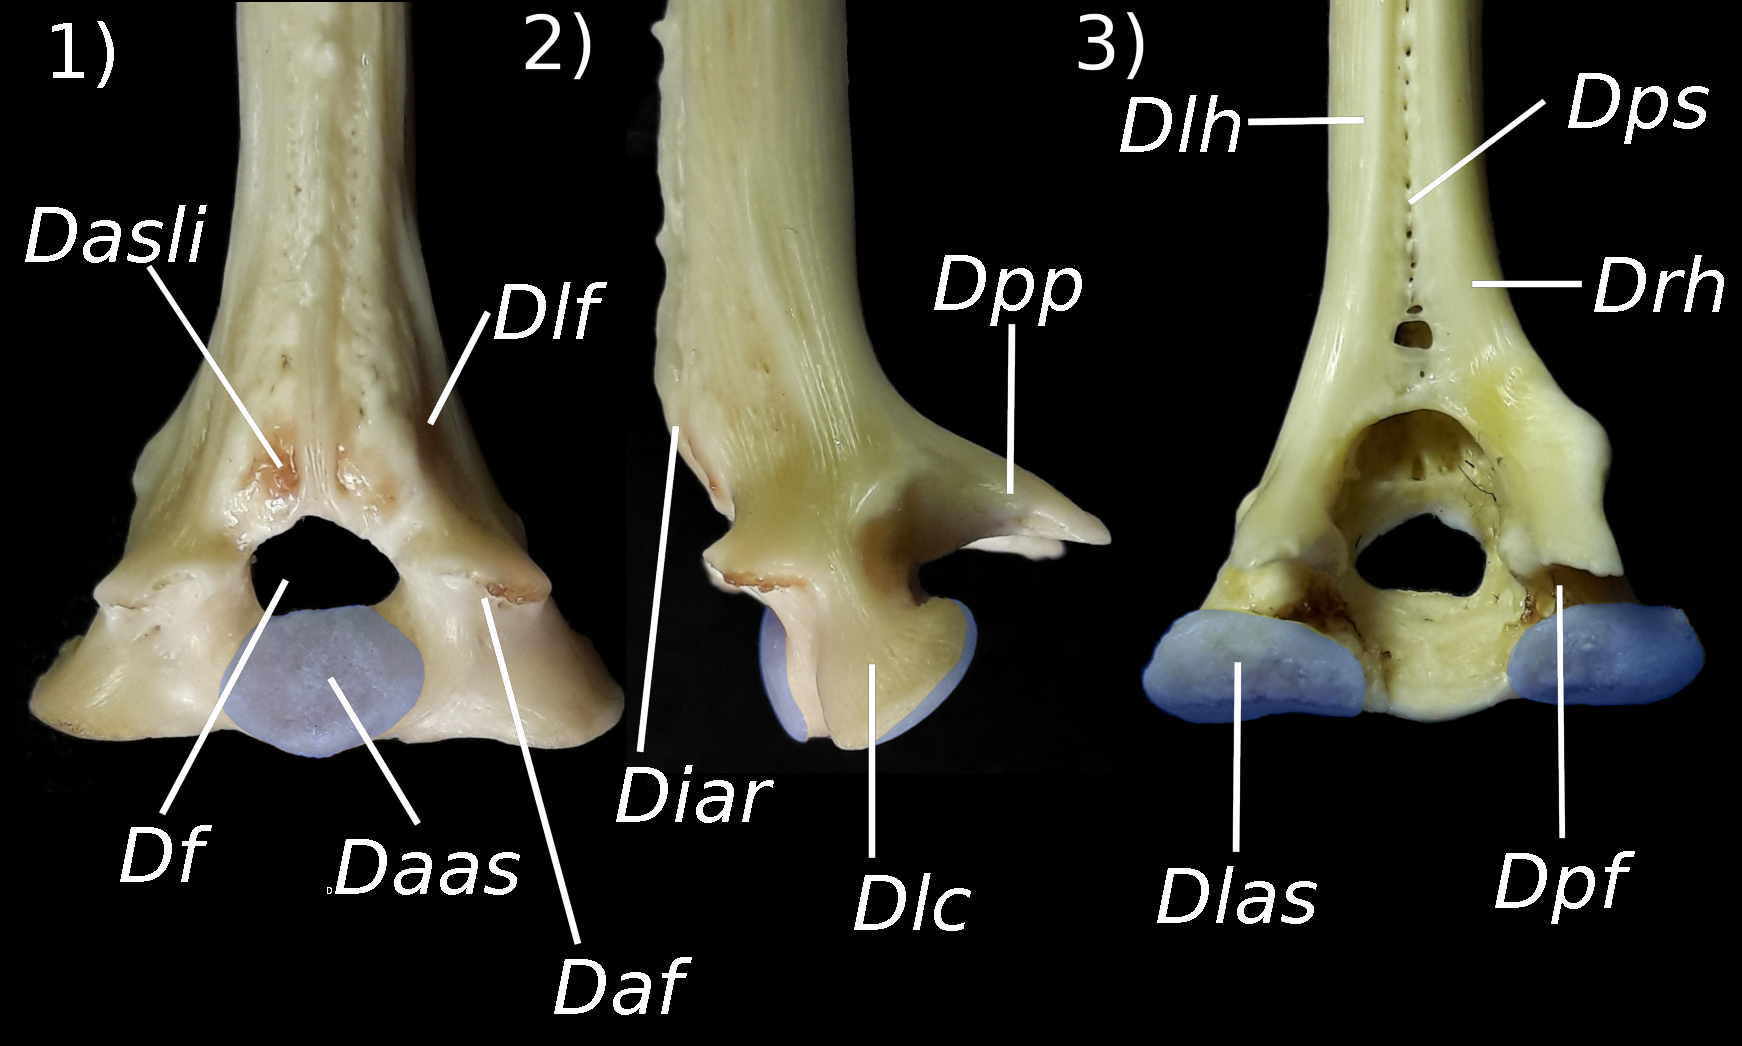
\includegraphics[width=\textwidth]{dorsal}
\caption{Legenda da figura}
\label{fig:dorsal}
\end{figure}

\section{Resultados}

Vivamus aliquet vitae nibh vel blandit. Mauris sed quam vel dui scelerisque pulvinar et in est. Pellentesque dignissim imperdiet libero in tincidunt. Fusce posuere fermentum justo, ac faucibus augue cursus vitae. Ut dictum vulputate metus, ac semper metus volutpat vitae. Morbi est nibh, consectetur vel ante sit amet, imperdiet venenatis quam. Nulla dictum quam eu orci maximus, vel faucibus magna placerat. Nullam libero est, tincidunt bibendum condimentum sed, rhoncus sit amet nulla. Vestibulum at mauris lobortis, malesuada leo in, viverra justo. Aliquam iaculis laoreet est vel faucibus. Donec faucibus orci ac turpis blandit maximus. Nulla semper laoreet lorem, ultrices pulvinar sem tristique eu. Vivamus vel cursus felis, sit amet euismod arcu. Sed sit amet ipsum volutpat, eleifend erat ut, vehicula nulla. Sed viverra nisi sollicitudin, elementum elit sed, suscipit leo. Nulla pulvinar metus at malesuada pretium. 

\section{Discusão}

As tabelas tem uma sintaxe particular, como na Tabela \ref{tab:tabelaExemplos}

\begin{table}
\begin{center}
\caption{O titulo das tabelas geralmente debe se posicionar encima da tabela} \label{tab:tabelaExemplos}
    \begin{tabular}{ | l | l | l | p{5cm} |}
    \hline
    Day & Min Temp & Max Temp & Summary \\ \hline
    Monday & 11C & 22C & A clear day with lots of sunshine.  
    However, the strong breeze will bring down the temperatures. \\ \hline
    Tuesday & 9C & 19C & Cloudy with rain, across many northern regions. Clear spells 
    across most of Scotland and Northern Ireland, 
    but rain reaching the far northwest. \\ \hline
    Wednesday & 10C & 21C & Rain will still linger for the morning. 
    Conditions will improve by early afternoon and continue 
    throughout the evening. \\
    \hline
    \end{tabular}
\end{center}
\end{table}

\bibliographystyle{palelec} % citação bibliográfica segundo o formato da revista Palaeontologia Electronica
\bibliography{refs/BiblioTese}  % associado ao arquivo: BiblioTese.bib'            % texto do capitulo dois, no arquivo capitulo2.tex

% cabeçalho para os apêndices
\renewcommand{\chaptermark}[1]{\markboth{\MakeUppercase{\appendixname\ \thechapter}} {\MakeUppercase{#1}} }
\fancyhead[RE,LO]{}

\appendix

\chapter{Material examinado}
\label{app:appMaterialExamined}

\textbf{AUCHENIPTERIDAE}

\textit{Ageneiosus pardalis}: ICNMHN 10014. \textit{Liosomadoras morrowi}: ICNMHN 14026. \textit{Tetranematichthys quadrifilis}: ICNMHN 12385. \textit{Trachelyopterichthys anduzei}: ICNMHN 16904. \textit{Trachelyopterus insignis}: ICNMHN uncat. \textit{Trachycorystes trachycorystes}: ICNMHN 2761.

\textbf{DIPLOMYSTIDAE}

\textit{Diplomystes viedmensis}: ANSP 192904.

\textbf{DORADIDAE}

\textit{Acanthodoras spinosissimus}: ICNMHN 8266. \textit{Agamyxis albomaculatus}: ICNMHN 1319. \textit{Amblydoras} cf. \textit{affinis}: ICNMHN 8287. \textit{Anadoras grypus}: ICNMHN 8274. \textit{Centrochir crocodili}: ICNMHN 5698. \textit{``Doras'' punctatus}: ICNMHN 16705. \textit{Hemidoras stenopeltis}: ICNMHN 5936. \textit{Hypodoras forficulatus}: ICNMHN 10143. \textit{Leptodoras} cf. \textit{nelsoni}: ICNMHN 413. \textit{Leptodoras} sp.: ICNMHN 8422. \textit{Megalodoras uranoscopus}: ICNMHN 6996. \textit{Nemadoras elongatus}: ICNMHN 8399. \textit{Opsodoras stubelli}: ICNMHN 17104. \textit{Orinocodoras eigenmanni}: ICNMHN 8441. \textit{Oxydoras niger}: ICNMHN 8445. \textit{Platydoras armatulus}: ICNMHN 10025. \textit{Pterodoras granosus}: ICNMHN 8300. \textit{Rhinodoras thomersoni}: ICNMHN 2172. \textit{Scorpiodoras heckelii}: ICNMHN 12962

\textbf{HEPTAPTERIDAE}

\textit{Pimelodella chagresi}: ICNMHN 1623.

\textbf{PIMELODIDAE}

\textit{Bergiaria westermanni}: MZUSP 85627. \textit{Brachyplatystoma capapretum}: MZUSP 53262, ANSP 178524, 179733, 178524. \textit{Brachyplatystoma juruense}: ANSP 178514-1,3,4,6, DUF 1071. \textit{Brachyplatystoma platynemum}: DUF 993, 1076, ANSP uncat, 187321. \textit{Brachyplatystoma rousseauxii}: ANSP 179794, 179793, 179233, DUF 1051, 981, 1078. \textit{Brachyplatystoma vaillanti}: ANSP 179799, 178525, 179474, DUF 994, 1164. \textit{Brachyplaystoma filamentosum}: DUF 1079, 1080, ANSP 179776. \textit{Calophysus macropterus}: DUF 1199, 1049, 403, ANSP 199813, 178164, 178260, ICNMHN uncat. \textit{Duopalatinus emarginatus}: MZUSP 85622. \textit{Exallodontus aguanai}: ANSP 18947, uncat. \textit{Hemisorubim platyrhynchos}: ANSP uncat, 179234, ICNMHN 7909. \textit{Hypophthalmus} sp. ``curved'': ANSP uncat. \textit{Hypophthalmus} sp. ``straight'': ANSP 180993, 178512, 180993, 187103. \textit{Iheringichthys labrosus}: ANSP 180505, MZUSP 78459, uncat. \textit{Leiarius perruno}: ANSP uncat-I, uncat-II, ICNMHN 2158. \textit{Leiarius} sp.: ANSP 178526, 178527, uncat without skull, DUF 1054, 1056, 1036, 1055, 1037. \textit{Luciopimelodus pati}: ANSP 178798, MZUSP 78464, 78457. \textit{Megalonema platanum}: MZUSP 78465. \textit{Megalonema platycephalum}: ANSP 179249, 178515. \textit{Parapimelodus nigribarbus}: MZUSP 78451. \textit{Parapimelodus valenciennesi}: MZUSP 78466, ANSP 178800. \textit{Phractocephalus hemioliopterus}: ANSP 179559, 179553, 179554, ICN uncat. \textit{Pimelodina flavipinnis}: ANSP uncat, 178513, 178516. \textit{Pimelodus argenteus}: ANSP 181017, uncat. \textit{Pimelodus grosskopfii}: ICNMHN 6867. \textit{Pimelodus mysteriosus}: ANSP 180506. \textit{``Pimelodus'' ornatus}: ANSP 178452, 180985. \textit{Pinirampus argentinus}: ANSP 181016. \textit{Pinirampus pirinampu}: ANSP uncat, 178530. \textit{Platynematichthys notatus}: ANSP uncat, 178528. \textit{Platysilurus malarmo}: ANSP uncat. \textit{Platysilurus mucosus}: DUF 986, uncat, ANSP 178508, 178509. \textit{Platystomatichthys sturio}: ANSP uncat, SU 22463, ICNMHN 15201. \textit{Propimelodus} sp.: ANSP 180939. \textit{Pseudoplatystoma corruscans}: ANS 188913, MZUSP 78477. \textit{Pseudoplatystoma fasciatum}: ANSP 177346. \textit{Pseudoplatystoma magdaleniatum}: ICNMHN 6860. \textit{Pseudoplatystoma metense}: ANSP 149541. \textit{Pseudoplatystoma reticulatum}: ANSP 188912. \textit{Pseudoplatystoma} sp.: DUF 1125, ICNMHN uncat. \textit{Pseudoplatystoma tigrinum}: DUF 921, uncat, ANSP 187010. \textit{Sorubim cuspicaudus}: MBUCV uncat, DUF 932. \textit{Sorubim elongatus}: ICNMHN 15039. \textit{Sorubim lima}: ANSP 178507. \textit{Sorubim trigonocephalus}: ANSP 188824. \textit{Sorubimichthys planiceps}: 179235, 17850. \textit{Steindachneridion scripta}: MZUSP 78463. \textit{Zungaro zungaro}: ANSP uncat, DUF 982, ICN uncat. % apêndice no arquivo apeMaterialExaminado.tex

% ---------------------------------------------------------------------------- %
% Capitulo final com todas as referências do documento
% NOTE: ALWAYS RUN C-c C-c BibTex BEFORE C-c C-c LaTeX in order to compile the references! The output of mendeley is right
\backmatter \singlespacing   % espaçamento simples
\bibliographystyle{palelec} % citação bibliográfica segundo o estilo da revista Palaeontologia Electronica
\bibliography{refs/BiblioTese}  % associado ao arquivo: BiblioTese.bib'

% ---------------------------------------------------------------------------- %
% Index
\index{TBP|see{periodicidade região codificante}}
\index{DSP|see{processamento digital de sinais}}
\index{STFT|see{transformada de Fourier de tempo reduzido}}
\index{DFT|see{transformada discreta de Fourier}}
\index{Fourier!transformada|see{transformada de Fourier}}

\printindex   % imprime o índice remissivo no documento 

\end{document}
